% ============================================================
%  Sistema de Detección de Mensajes Fraudulentos
%  Formato LNCS — Lecture Notes in Computer Science
%  Autor: Camilo Humberto Pérez Fleita — Proyecto Final IA 2025–2026
% ============================================================
\documentclass{llncs}

\usepackage[T1]{fontenc}
\usepackage[utf8]{inputenc}
\usepackage[spanish]{babel}
\usepackage{booktabs}
\usepackage{amsmath,amssymb}
\usepackage{graphicx}
\usepackage{hyperref}
\usepackage{xcolor}
\usepackage{multirow}
\usepackage{array}

% Evitar que hyperref rompa las referencias cruzadas en LNCS
\hypersetup{hidelinks}

% ============================================================
\begin{document}
% ============================================================

\title{Sistema de Detección de Mensajes Fraudulentos\\
Mediante Cascada Multimodal con Metaheurísticas\\
y Análisis Conversacional}

\author{Camilo Humberto Pérez Fleita}

\institute{Facultad de Matemática y Computación, Grupo C312\\
Universidad de La Habana, Cuba\\
\email{camiloperezhf@gmail.com}}

\maketitle

% ============================================================
\begin{abstract}
Se presenta un sistema automatizado de detección de mensajes fraudulentos
motivado por la creciente proliferación de estafas digitales en Cuba
y diseñado para ser aplicable al contexto latinoamericano en general.
La arquitectura combina una cascada de nueve capas:
motor de reglas, clasificador LightGBM, detección de anomalías
con Isolation Forest, red bayesiana, razonamiento basado en casos,
embeddings semánticos (Mistral), modelo de lenguaje grande (Mistral),
meta-aprendiz por apilamiento y análisis conversacional con BiLSTM.
La optimización emplea cinco técnicas metaheurísticas:
PSO para hiperparámetros, Recocido Simulado y Búsqueda Tabú para
umbrales de la cascada, Simulación de Eventos Discretos para
generación de datos sintéticos y Optimización por Colonia de Hormigas
para la detección de arcos de manipulación.
El conjunto de datos comprende 5\,572 mensajes reales más 2\,118 sintéticos.
Resultados: LightGBM 98.21\,\% de exactitud, F1-fraude de 0.93;
meta-aprendiz AUC 0.9991; BiLSTM 91.37\,\%.
El sistema cuenta con 243 pruebas automatizadas.
\keywords{detección de fraude \and aprendizaje automático \and
cascada de clasificadores \and metaheurísticas \and
análisis conversacional \and LLM}
\end{abstract}

% ============================================================
\section{Introducción}
\label{sec:intro}
% ============================================================

El fraude mediante mensajes de texto y aplicaciones de mensajería
instantánea es, en esencia, un problema de ingeniería social:
el atacante no explota vulnerabilidades técnicas, sino la confianza
y la urgencia percibida de su víctima.
En Cuba, la rápida expansión del acceso a internet móvil y de
plataformas de compraventa digital como Revolico ha dado lugar
a una proliferación de estas estafas~\cite{almeida2011}:
vendedores ficticios que cobran por adelantado sin entregar el producto,
suplantación de compradores o vendedores legítimos, y conversaciones
diseñadas para generar confianza antes de solicitar transferencias
o datos personales.
El 13.4\,\% de los mensajes en el corpus empleado en este trabajo
son fraudulentos, proporción que refleja la frecuencia real del fenómeno.

Detectar automáticamente estos mensajes plantea un reto
que ningún modelo individual resuelve bien por sí solo.
Los métodos basados en palabras clave capturan los casos obvios
pero fallan ante variaciones ortográficas o sinónimos regionales;
los clasificadores de aprendizaje automático clásicos no modelan
el significado profundo del texto; y los modelos de lenguaje grande,
aunque comprenden el contexto con precisión, resultan demasiado
lentos y costosos para analizar cada mensaje en tiempo real.
Más importante aún: ninguno de estos enfoques por sí solo modela
la \emph{dimensión conversacional} del fraude, en la que la estafa
no está en un mensaje aislado sino en la secuencia completa de
turnos, donde el atacante construye confianza progresivamente
antes de revelar su intención real.

Este trabajo propone una \emph{cascada multimodal} de nueve capas
como respuesta a este conjunto de limitaciones.
La idea central es sencilla: los casos más evidentes se resuelven
rápido y barato en las primeras capas; solo los mensajes ambiguos
escalan hasta las capas más potentes y costosas.
Así se obtiene la precisión de un modelo de lenguaje grande sin
pagar su costo computacional en el 100\,\% de los casos.

Las contribuciones principales son:
\begin{enumerate}
  \item Una cascada configurable de nueve capas con puertas de cortocircuito
        que equilibra precisión y eficiencia computacional.
  \item Cinco técnicas metaheurísticas integradas para la optimización
        automática de hiperparámetros y umbrales en tiempo de ejecución.
  \item Un simulador de eventos discretos (DES) que genera conversaciones
        sintéticas de fraude con coherencia narrativa para ampliar el
        conjunto de entrenamiento del análisis conversacional.
  \item Un sistema de umbrales configurable en tiempo de ejecución
        que permite adaptar el comportamiento sin reentrenamiento.
\end{enumerate}

% ============================================================
\section{Caso de Uso Motivador: Estafa por Suplantación de Identidad}
\label{sec:casouse}
% ============================================================

Para ilustrar qué hace el sistema antes de describir cómo lo hace,
presentamos un caso real extraído del conjunto de imágenes de validación.
Se trata de una conversación de WhatsApp en la que el estafador suplanta
la identidad de un tercero conocido por la víctima ---presentando su
perfil, correo y nombre como respaldo de legitimidad--- para solicitar
el pago de un supuesto servicio y, en el proceso, obtener datos
personales de la víctima.

Este tipo de fraude es especialmente difícil de detectar con herramientas
de análisis léxico: el vocabulario de cada mensaje por separado es
perfectamente inocuo.
La señal de peligro no está en las palabras sino en la \emph{estructura
temporal de la conversación}: construcción de confianza inicial,
introducción gradual de una narrativa de pago y escalada de presión
hacia el cierre de la transacción.

\subsection*{Entrada: capturas de pantalla de la conversación}

El sistema acepta tanto texto plano como imágenes.
Cuando el usuario sube capturas de pantalla, el módulo de visión
(Pixtral-12b) extrae el texto de cada imagen mediante OCR y lo
incorpora como mensajes numerados al pipeline de análisis.
La Figura~\ref{fig:upload} muestra la pantalla de carga con los tres
pantallazos de la conversación.

\begin{figure}[ht]
\centering
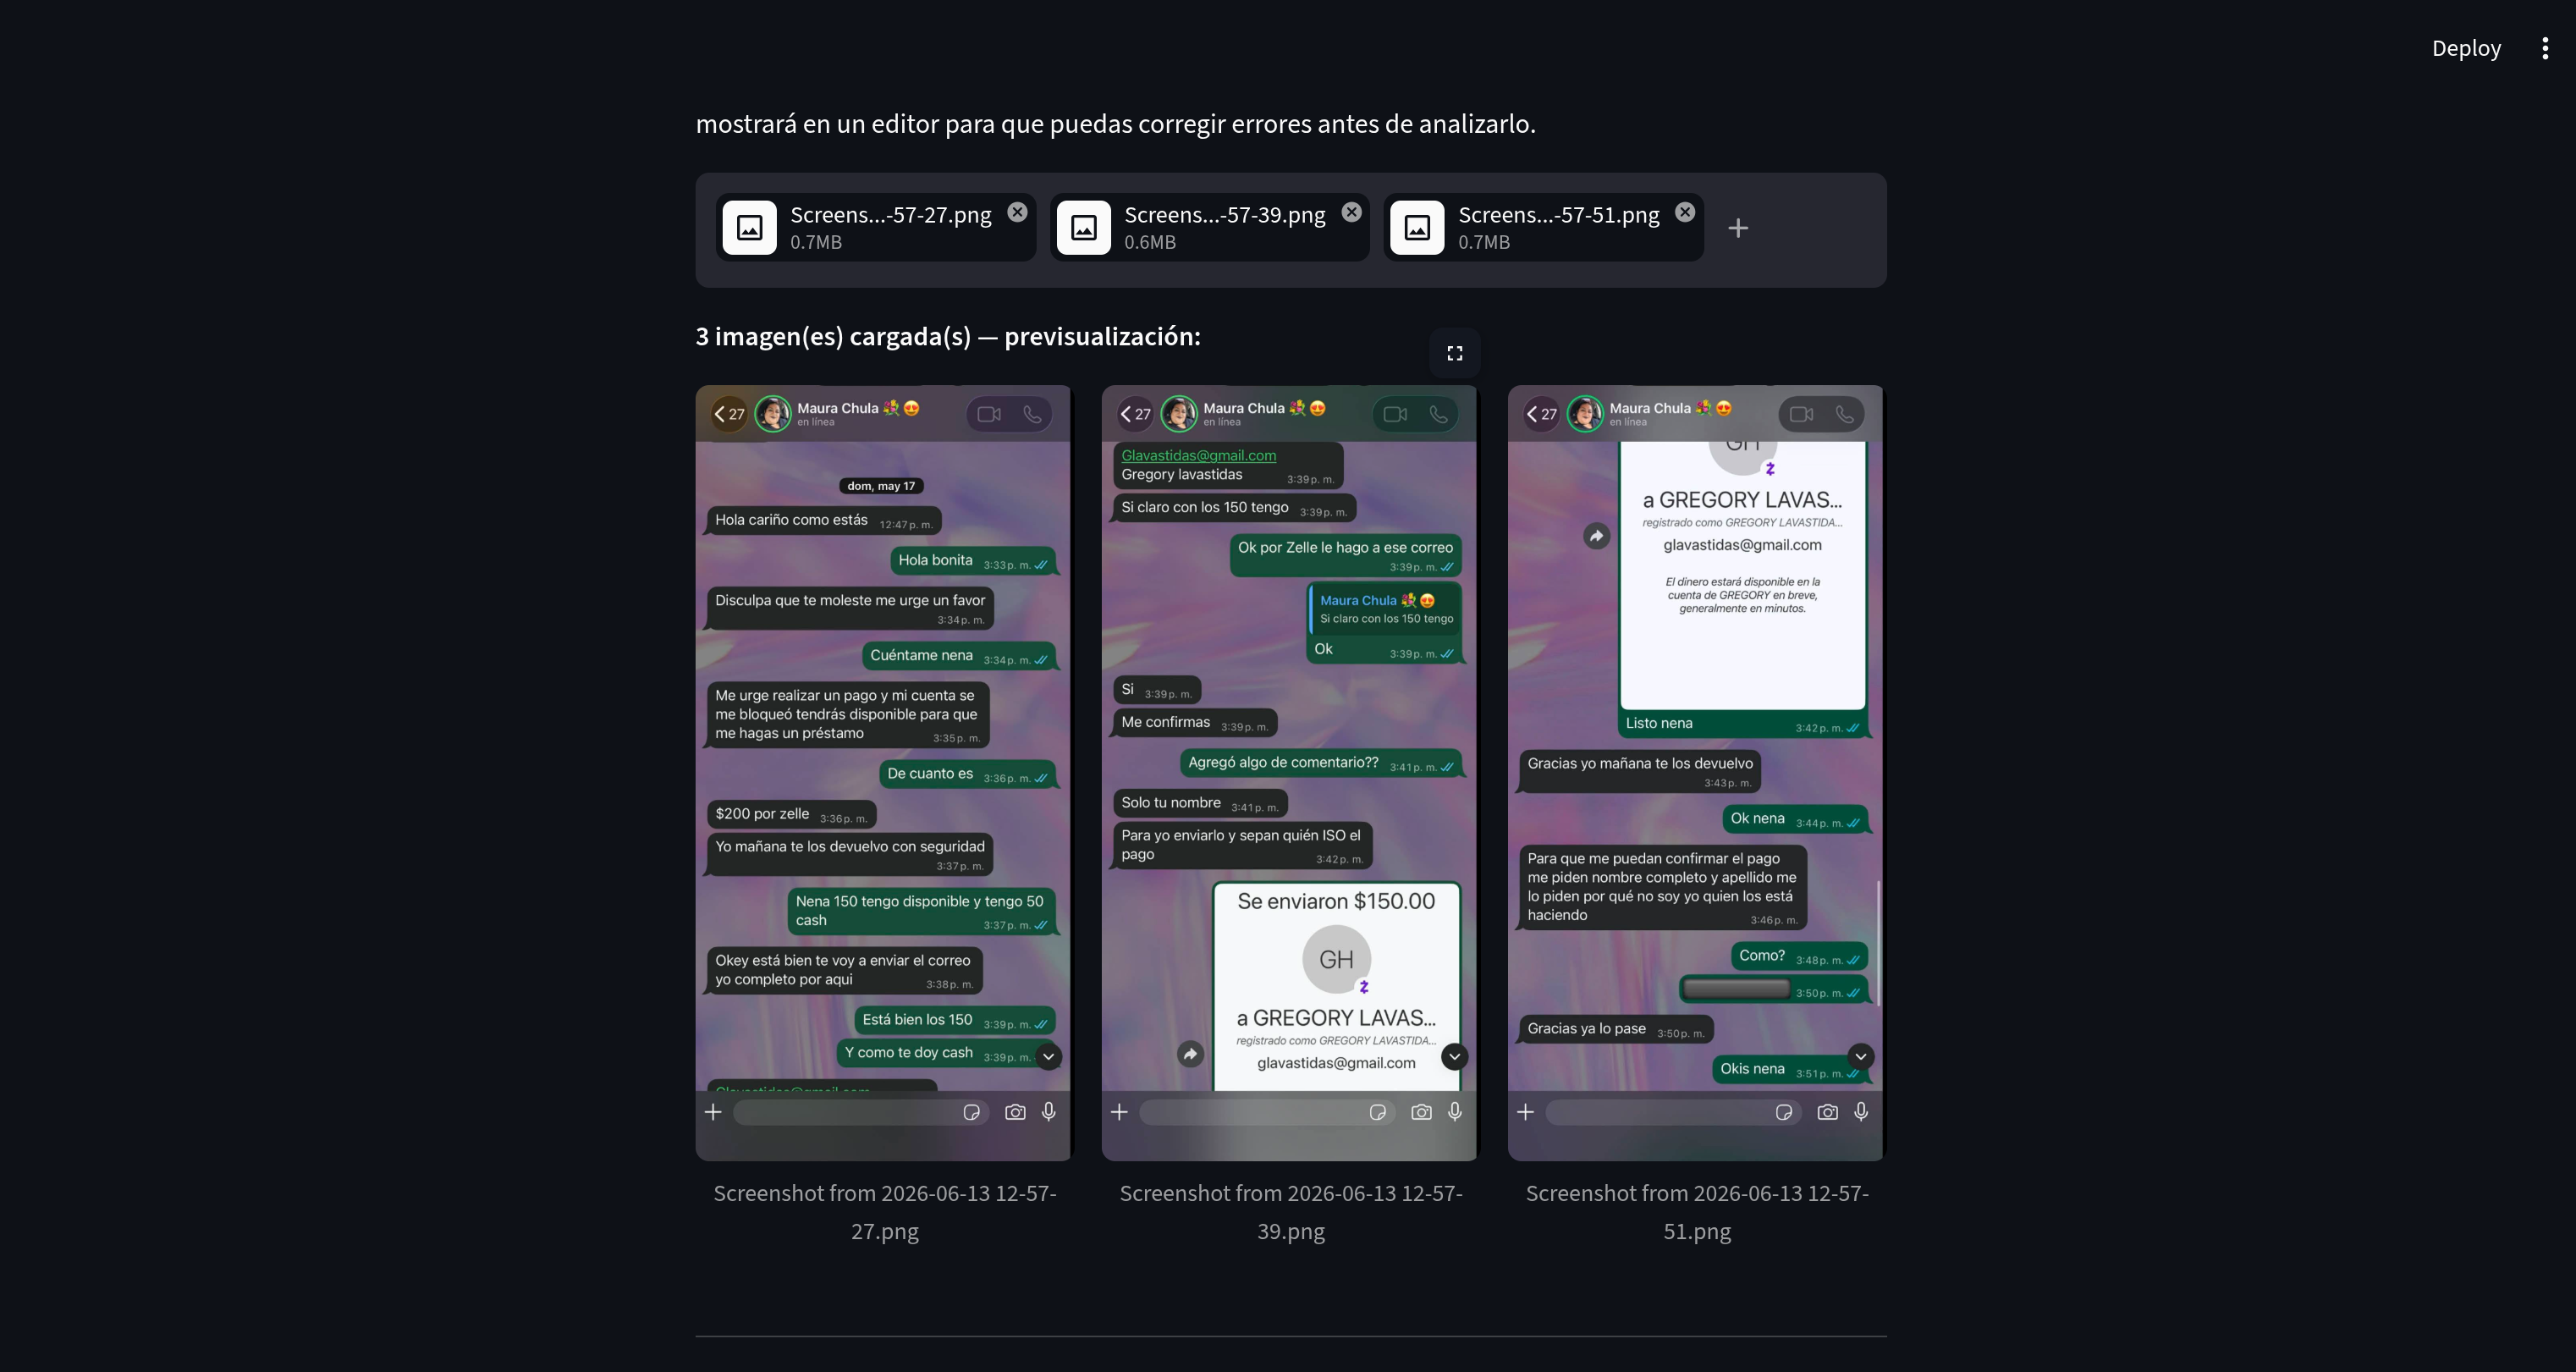
\includegraphics[width=\textwidth]{../assets/1}
\caption{Carga de tres capturas de pantalla de WhatsApp.
  La conversación involucra una cuenta \emph{(Maura Chula)} que presenta
  la identidad de un tercero \emph{(Gregory Lavas)} ---con perfil, correo
  y nombre completo--- como garantía de solvencia para el pago de
  un servicio.}
\label{fig:upload}
\end{figure}

La mecánica concreta del fraude se desarrolla en tres actos.
Primero, la cuenta contactante presenta el perfil completo de una tercera
persona ---nombre, correo y fotografía--- como prueba de que la
operación es real y que existe un respaldo detrás de la solicitud.
Segundo, negocia un monto concreto (150 unidades disponibles más 50 en
efectivo) enmarcándolo como el pago de un servicio, no como una
petición de dinero directa, lo que reduce la alerta de la víctima.
Tercero, una vez acordado el monto, solicita el correo electrónico de
la víctima con el pretexto de ``enviar la información completa''.
El objetivo real de esa última petición no es cerrar el pago:
es obtener datos de contacto personales que serán explotados en
comunicaciones fraudulentas posteriores.

\subsection*{Resultado: panel de riesgo global}

Tras el análisis de los 30 mensajes extraídos mediante OCR, el sistema
emite el veredicto mostrado en la Figura~\ref{fig:dashboard}.

\begin{figure}[ht]
\centering
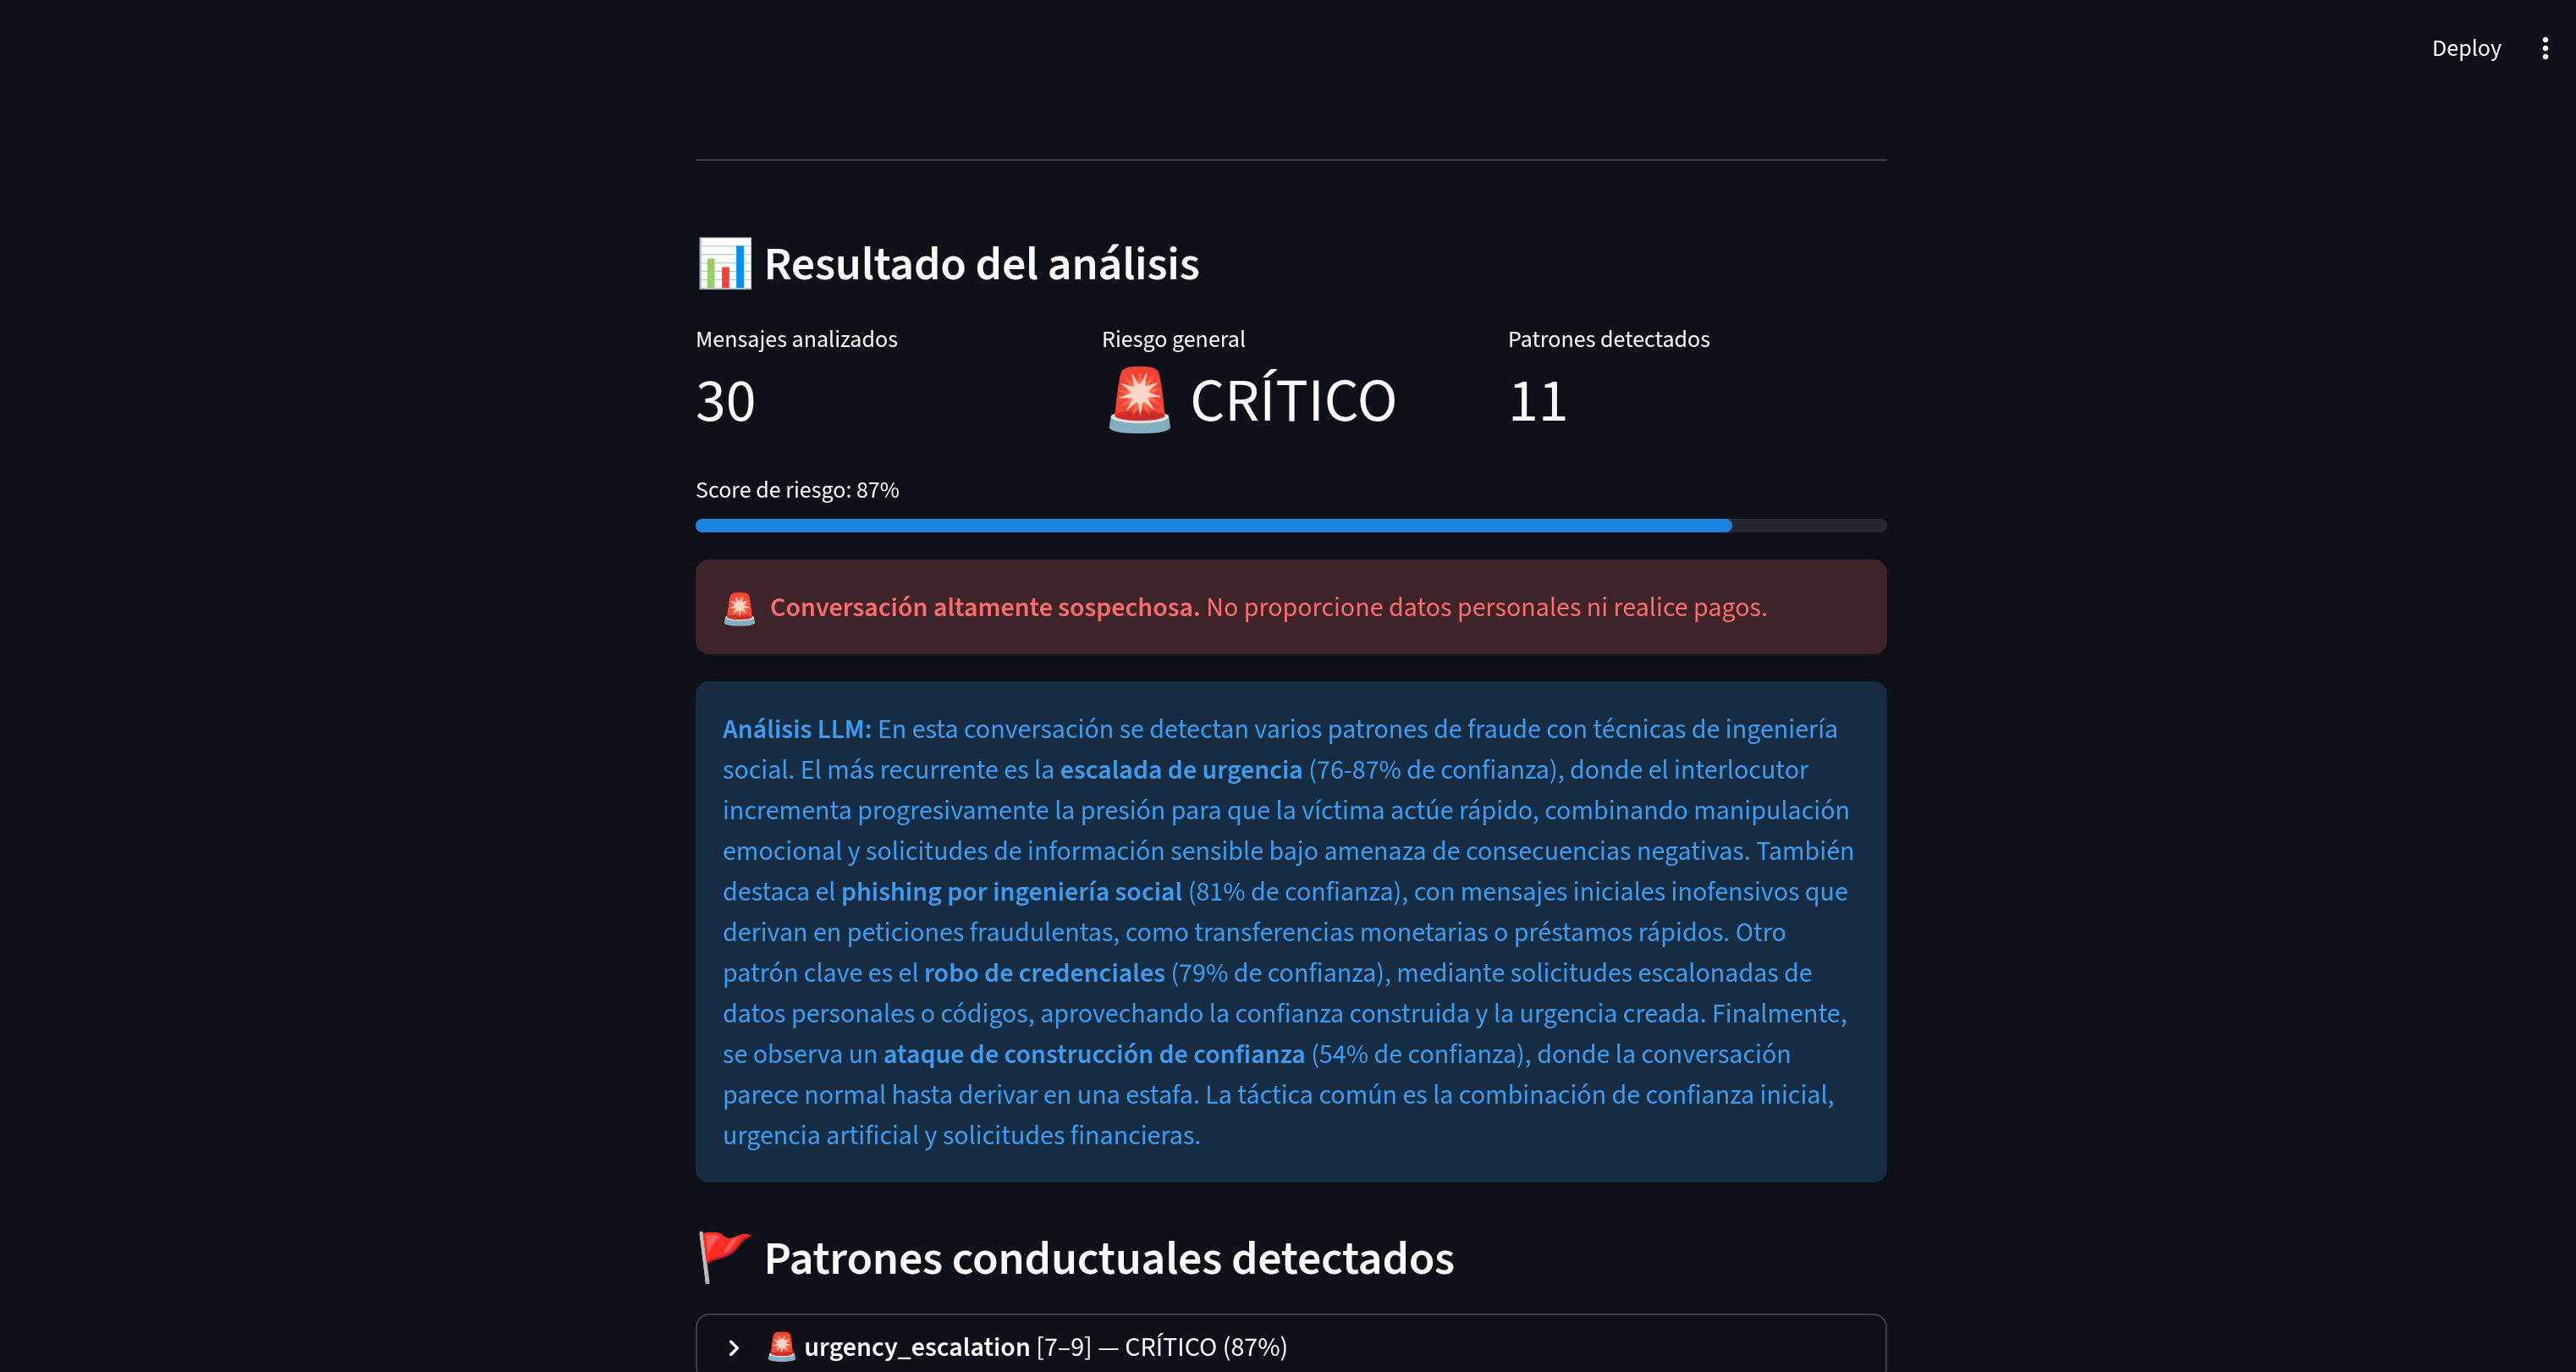
\includegraphics[width=\textwidth]{../assets/3}
\caption{Panel de resultado. 30 mensajes analizados, riesgo
  \textbf{CRÍTICO} (87\,\%), 11 patrones conductuales detectados.
  El análisis LLM identifica la escalada de urgencia artificial,
  el phishing por ingeniería social y el robo de credenciales
  como los tres ejes principales de la estrategia fraudulenta.}
\label{fig:dashboard}
\end{figure}

El sistema no se limita a emitir una etiqueta binaria.
El campo \emph{Análisis LLM} articula en lenguaje natural la estrategia
completa del estafador: mensajes iniciales inofensivos que construyen
confianza, escalada artificial de urgencia para presionar a la víctima
a actuar sin reflexionar, y solicitud escalonada de datos sensibles
aprovechando la confianza ya creada.
El sistema genera además una advertencia concreta dirigida al usuario:
\emph{``No proporcione datos personales ni realice pagos''},
formulada en lenguaje directo y accionable en lugar de limitarse
a reportar un score numérico.

\subsection*{Detalle: patrones conductuales por rango de mensajes}

La capa de análisis conversacional no solo nombra los patrones
detectados sino que los localiza en el rango exacto de mensajes
donde se manifiestan.
La Figura~\ref{fig:patterns} muestra los cinco patrones con mayor
nivel de confianza.

\begin{figure}[ht]
\centering
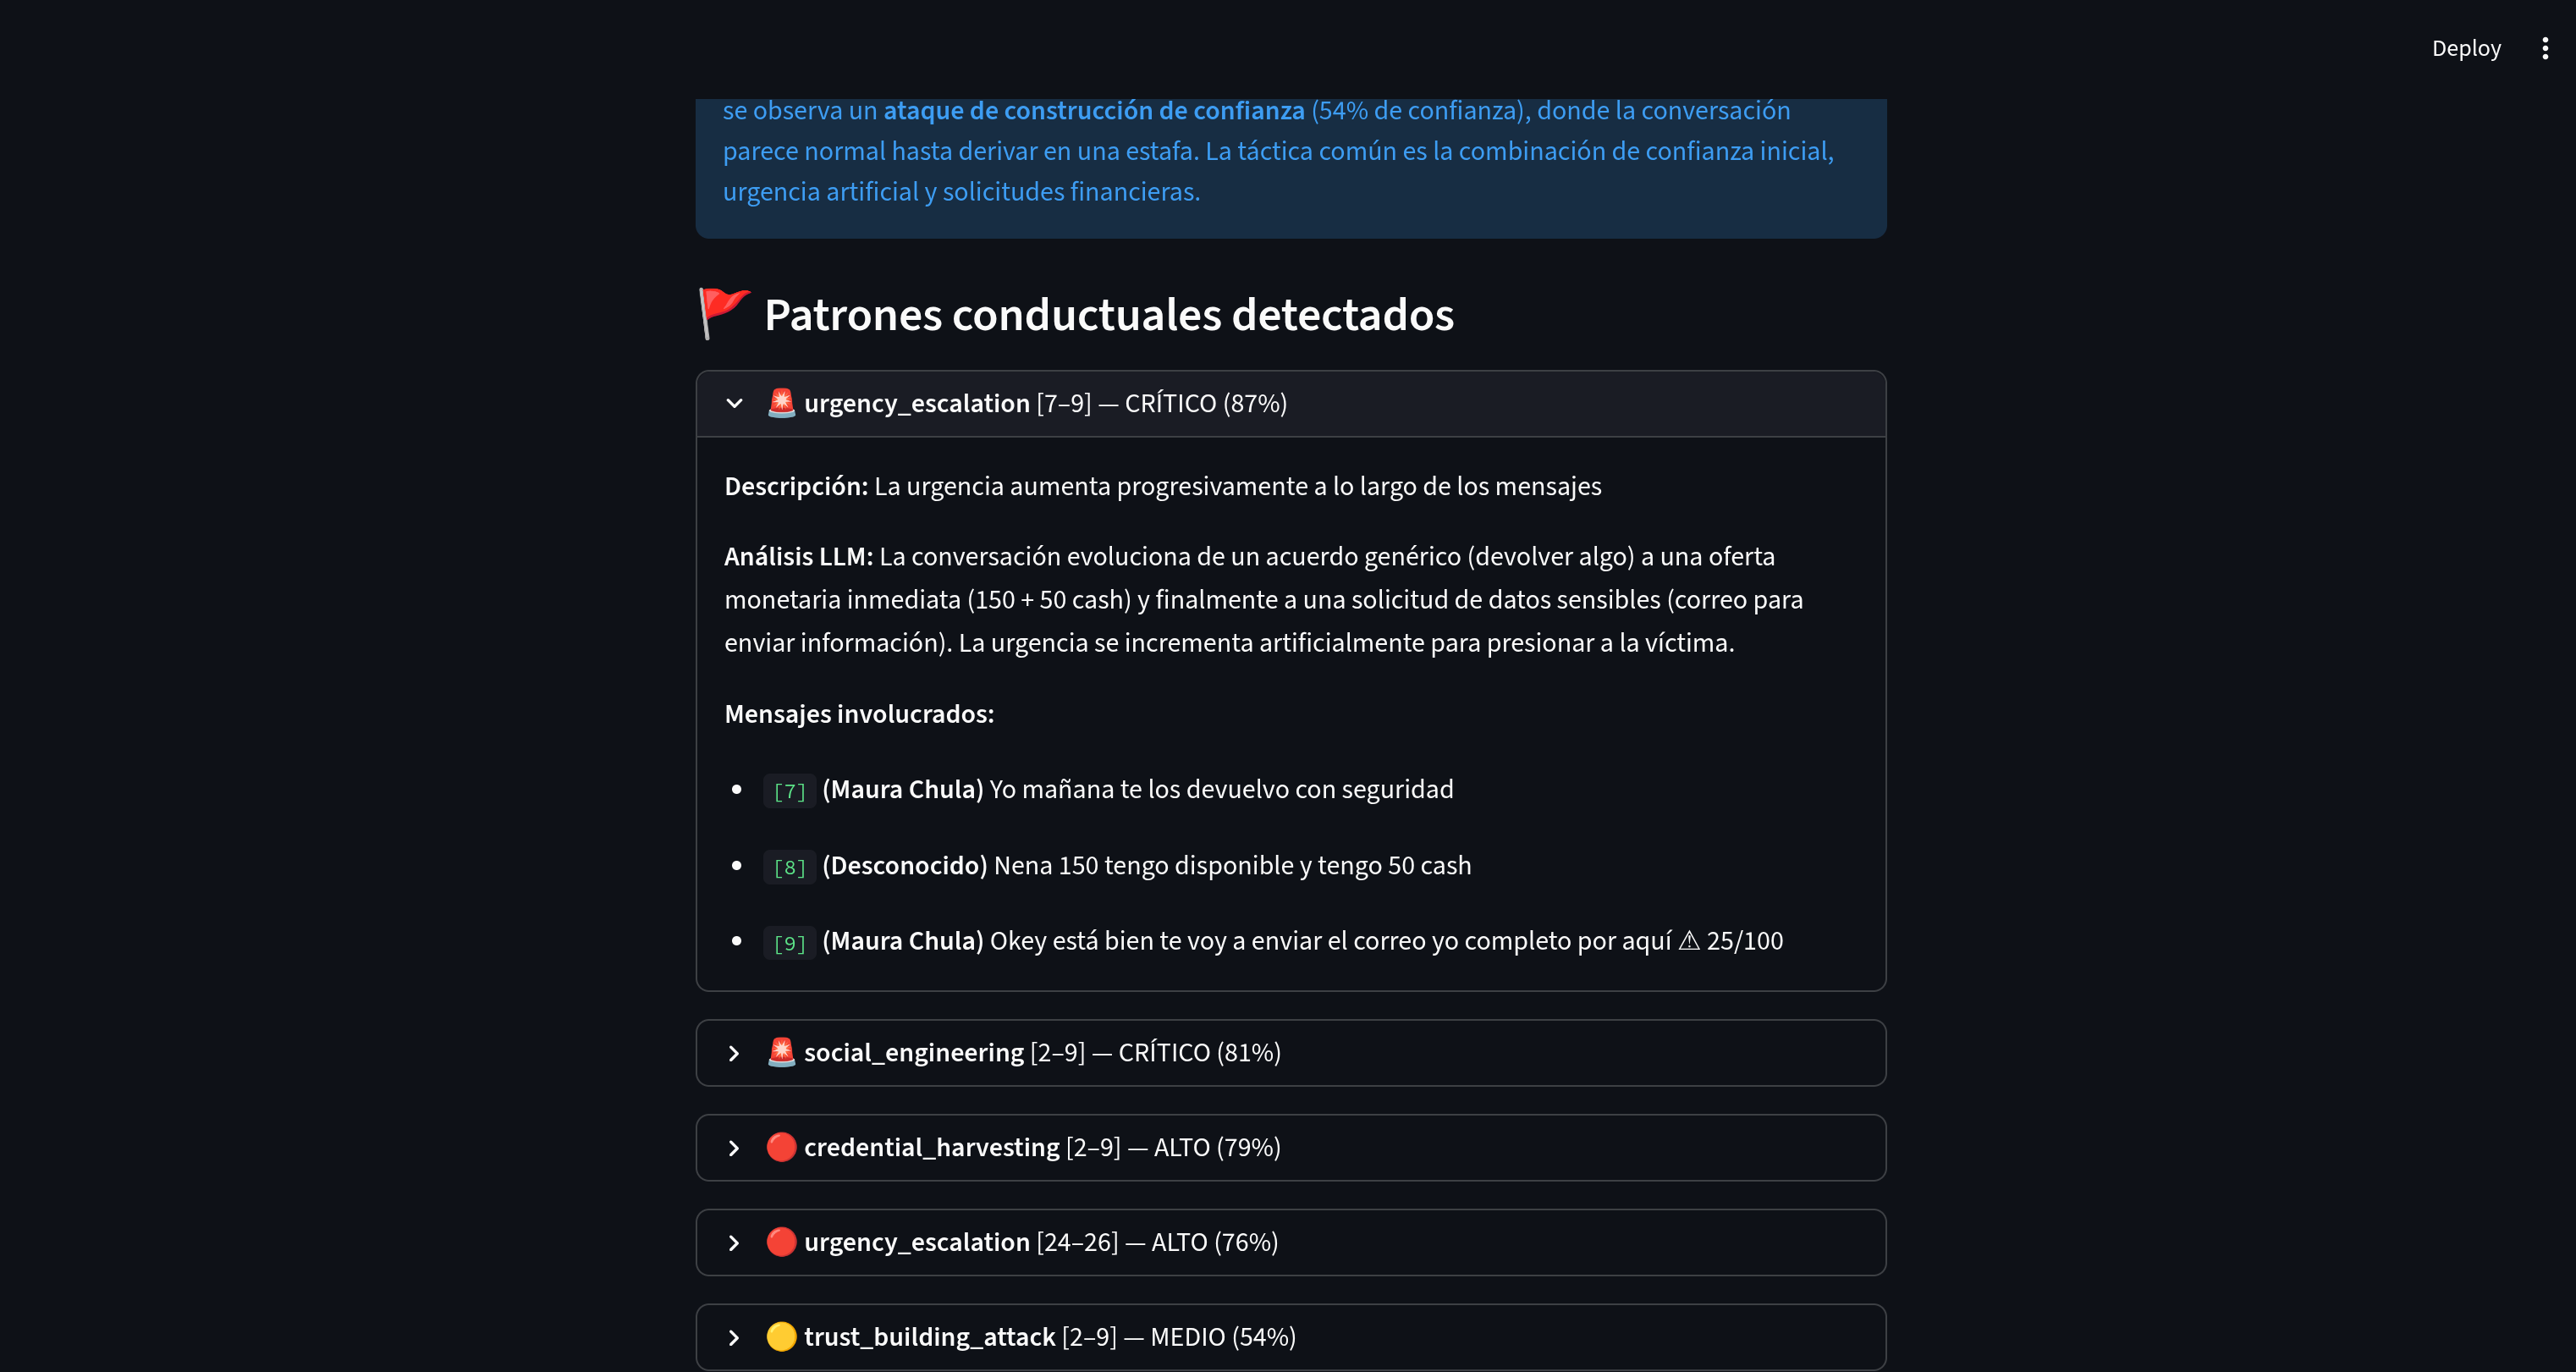
\includegraphics[width=\textwidth]{../assets/2}
\caption{Patrones conductuales detectados por rango de mensajes.
  \texttt{urgency\_escalation} [7--9] alcanza 87\,\% de confianza
  y engloba el bloque donde se negocia el monto y se solicita el
  correo. \texttt{social\_engineering} [2--9] (81\,\%) cubre la
  fase completa de suplantación. \texttt{credential\_harvesting}
  [2--9] (79\,\%) captura la extracción de datos personales.
  El nivel \textsc{CRÍTICO} se activa cuando al menos dos patrones
  de alta confianza coexisten en rangos solapados.}
\label{fig:patterns}
\end{figure}

El desglose por rango de mensajes revela la \emph{anatomía temporal}
del fraude: la suplantación de identidad opera desde el mensaje~2,
la ingeniería social se sostiene durante toda la conversación, y la
presión máxima ---urgencia escalada más solicitud de datos--- converge
en el bloque [7--9].
Esto permite al analista o a la propia víctima identificar el punto
exacto en que la conversación dejó de ser legítima sin necesidad de
revisar los 30 mensajes manualmente.
La combinación de veredicto global (Figura~\ref{fig:dashboard}) con
localización de patrones (Figura~\ref{fig:patterns}) es lo que
distingue al sistema de un clasificador binario convencional y lo
convierte en una herramienta de apoyo a la decisión.

% ============================================================
\section{Trabajos Relacionados}
\label{sec:related}
% ============================================================

La detección de spam en SMS tiene como referencia fundacional el
trabajo de Almeida et al.~\cite{almeida2011}, que estableció el
SMS Spam Collection Dataset y evaluó clasificadores Naïve Bayes
con características de bolsa de palabras, obteniendo precisiones
superiores al 97\,\%.
Aunque el dataset fue concebido en inglés, su metodología influyó
decisivamente en trabajos posteriores para español.

Para phishing por correo electrónico, los modelos SVM con núcleos
RBF~\cite{cortes1995} dominaron la literatura durante varios años,
complementados con características de la URL y metadatos del
encabezado del correo.
Fette et al.\ demostraron que las características estructurales
del mensaje superan a las puramente léxicas~\cite{fette2007},
anticipando la necesidad de análisis más allá del vocabulario.

Con la aparición de los modelos de lenguaje grande, varios trabajos
han explorado su uso directo para clasificación de fraude.
Jiang et al.\ demostraron que Mistral 7B, mediante prompting
estructurado en JSON, produce clasificaciones de alta fidelidad
con explicaciones interpretables~\cite{jiang2023mistral}.
Sin embargo, la latencia y el costo de invocar un LLM por cada
mensaje hacen inviable su uso indiscriminado en producción,
motivando precisamente la arquitectura en cascada de este trabajo.

El análisis conversacional del fraude es un área más reciente.
Las arquitecturas BiLSTM con atención han mostrado efectividad
en la detección de patrones secuenciales en diálogos de soporte
técnico fraudulento~\cite{hochreiter1997}, capturando dependencias
temporales que los modelos por mensaje individual no pueden ver.

Nuestro trabajo se distingue por combinar todos estos enfoques
en una cascada unificada con puertas de cortocircuito, añadiendo
optimización metaheurística de los umbrales y un simulador DES
para generación de datos sintéticos conversacionales.
Esta combinación no tiene precedentes directos en la literatura
de detección de fraude en español.

% ============================================================
\section{Arquitectura del Sistema}
\label{sec:arch}
% ============================================================

\subsection{Visión General de la Cascada}
\label{sec:arch:cascade}

Piénsese en la cascada como un sistema de filtros sucesivos.
El primer filtro es el más simple: un conjunto de reglas que
busca señales obvias (URLs, palabras de urgencia, solicitudes
de credenciales).
Si ese filtro es suficientemente seguro, el mensaje sale de la
cascada de inmediato.
Si no, pasa al siguiente filtro, progresivamente más sofisticado,
hasta llegar al análisis de lenguaje natural profundo.
Las \emph{puertas de cortocircuito} son los mecanismos que deciden
cuándo un filtro es suficientemente seguro como para no necesitar
el siguiente.

Formalmente, la cascada se puede expresar como:

\begin{equation}
  \mathcal{C} = G_2 \circ \mathrm{LLM} \circ G_1 \circ \mathrm{EMB}
    \circ \bigl(\mathrm{ML} \oplus \mathrm{ANO} \oplus \mathrm{BAY}
    \oplus \mathrm{CBR}\bigr) \circ \mathrm{REG}
  \label{eq:cascade}
\end{equation}

donde $\oplus$ denota ejecución en paralelo, $\circ$ es composición
secuencial y $G_k$ son las puertas de cortocircuito.

\textbf{Puerta 1 ($G_1$):}
Si la confianza del modelo ML es muy alta
($\mathrm{conf}_{\mathrm{ML}} \geq \theta_{g1}$)
\emph{y} la capa de reglas concuerda en sentido (ambas clasifican igual),
entonces los pasos más costosos —embeddings semánticos y LLM—
se omiten y se pasa directamente al meta-aprendiz.

\textbf{Puerta 2 ($G_2$):}
Si la similitud con el índice semántico es suficientemente clara
($\mathrm{sim}_{\mathrm{fraude}} \geq \theta_{\mathrm{emb}}$
o $\mathrm{sim}_{\mathrm{leg\acute{i}timo}} \geq \theta_{\mathrm{emb}}$),
entonces la llamada al LLM externo se evita.

\textbf{Meta-aprendiz:}
Al final de la cascada, todas las señales intermedias se combinan
con pesos aprendidos automáticamente:

\begin{equation}
  \hat{y} = f_{\mathrm{meta}}\!\left(
    [p_{\mathrm{ML}},\; r_{\mathrm{rule}},\; e_f,\; e_l,\;
     a,\; t,\; b,\; s_{\mathrm{cbr}}]
  \right)
  \label{eq:meta}
\end{equation}

donde $p_{\mathrm{ML}}$ es la probabilidad del clasificador LightGBM,
$r_{\mathrm{rule}}$ el puntaje normalizado del motor de reglas,
$e_f$ y $e_l$ las similitudes de embedding con las clases fraude y
legítimo respectivamente, $a$ el puntaje de anomalía,
$t$ la confianza del LLM, $b$ la probabilidad bayesiana y
$s_{\mathrm{cbr}}$ el puntaje de razonamiento basado en casos.

\subsection{Espacio de Características}
\label{sec:arch:features}

Antes de que cualquier modelo tome una decisión, cada mensaje se
convierte en un vector numérico.
Este proceso de \emph{vectorización} es el puente entre el texto
libre y los algoritmos matemáticos: transforma palabras en números
que los modelos pueden procesar.
Se emplean dos tipos de características complementarias que juntas
forman el vector $\phi(m) \in \mathbb{R}^{10\,017}$:

\begin{equation}
  \phi(m) = \bigl[\phi_{\mathrm{tfidf}}(m) \;\|\; \phi_{\mathrm{manual}}(m)\bigr]
  \label{eq:features}
\end{equation}

\textbf{Características TF-IDF} ($\mathbb{R}^{10\,000}$):
El modelo TF-IDF asigna a cada n-grama un peso proporcional a
cuánto aparece en el mensaje pero inversamente proporcional a
cuántos mensajes del corpus lo contienen; es decir, una palabra
que aparece mucho en fraudes pero poco en mensajes legítimos
recibirá un peso alto, y viceversa.
Se emplean $n$-gramas de 1 a 3 palabras,
\texttt{sublinear\_tf=True} y vocabulario de 10\,000 términos.

\textbf{Características manuales} ($\mathbb{R}^{17}$):
Complementan el TF-IDF con señales estructurales que no dependen
del vocabulario concreto: presencia de URLs, menciones de dinero,
signos de exclamación, proporción de mayúsculas.
La detección de negación emplea una ventana deslizante de 5 tokens
para capturar patrones como
``\emph{no es necesario que proporcione su contraseña}''
(donde la palabra ``contraseña'' resulta sospechosa solo en ausencia
de la negación).
Las 17 características se detallan en la Tabla~\ref{tab:features}.

\begin{table}[t]
\caption{Características manuales en $\phi_{\mathrm{manual}}(m)$.}
\label{tab:features}
\centering
\begin{tabular}{lll}
\toprule
Característica & Tipo & Descripción \\
\midrule
\texttt{msg\_length}         & entero  & Longitud en caracteres \\
\texttt{word\_count}         & entero  & Número de palabras \\
\texttt{has\_url}            & binario & Presencia de URL \\
\texttt{has\_email}          & binario & Presencia de e-mail \\
\texttt{has\_phone}          & binario & Presencia de teléfono \\
\texttt{has\_money}          & binario & Mención de cantidades monetarias \\
\texttt{exclamation\_count}  & entero  & Signos de exclamación \\
\texttt{question\_count}     & entero  & Signos de interrogación \\
\texttt{uppercase\_ratio}    & real    & Proporción de mayúsculas \\
\texttt{has\_urgency}        & binario & Palabras de urgencia \\
\texttt{has\_credential\_words} & binario & Palabras de solicitud de credenciales \\
\texttt{has\_prize\_words}   & binario & Palabras relacionadas con premios \\
\texttt{avg\_word\_length}   & real    & Longitud media de palabra \\
\texttt{has\_bank\_mentions} & binario & Mención de entidades bancarias \\
\texttt{negation\_score}     & real    & Puntaje de negación (ventana 5) \\
\texttt{entity\_count}       & entero  & Entidades nombradas detectadas \\
\texttt{has\_amount\_ner}    & binario & Cantidades detectadas por NER \\
\bottomrule
\end{tabular}
\end{table}

% ============================================================
\section{Modelos de Aprendizaje Automático}
\label{sec:ml}
% ============================================================

Con el vector de características construido, el sistema puede ya
aplicar modelos de aprendizaje automático.
Este trabajo emplea cuatro tipos de modelos en paralelo, cada uno
aportando una perspectiva distinta sobre el mensaje: uno que aprende
patrones estadísticos, uno que detecta lo que no debería existir,
uno que razona sobre combinaciones de señales y uno que busca
casos similares en la memoria del sistema.

\subsection{Modelo Base: LightGBM}
\label{sec:ml:lgbm}

El primero y más importante es LightGBM, un clasificador de
\emph{gradient boosting}.
La idea intuitiva del boosting es la de un comité de expertos débiles
que aprenden de sus errores mutuos: el primer árbol de decisión
clasifica todos los mensajes y se equivoca en algunos;
el segundo árbol se concentra especialmente en corregir esos errores;
el tercero corrige los errores del segundo, y así sucesivamente
hasta construir un clasificador fuerte.
LightGBM implementa esto de manera muy eficiente mediante histogramas,
lo que lo hace especialmente adecuado para vectores de alta dimensión
como los 10\,017 features de este trabajo.

El conjunto de datos presenta un desbalance significativo:
87\,\% de mensajes legítimos frente a 13\,\% fraudulentos.
Se emplea \texttt{class\_weight=``balanced''} para que LightGBM
ajuste automáticamente los pesos de clase sin submuestreo,
preservando la distribución natural.

La Tabla~\ref{tab:ml} compara los clasificadores evaluados.
LightGBM obtiene la mayor exactitud (98.21\,\%) y F1-fraude (0.93).

\begin{table}[t]
\caption{Comparativa de clasificadores sobre el conjunto de prueba
(80/20 estratificado).}
\label{tab:ml}
\centering
\begin{tabular}{lrrrrr}
\toprule
Modelo & Exactitud & Precisión & Recall & F1-fraude & F1-ponderado \\
\midrule
Regresión Logística & 0.9731 & 0.89 & 0.91 & 0.90 & 0.9729 \\
Random Forest       & 0.9758 & 0.91 & 0.90 & 0.90 & 0.9755 \\
XGBoost             & 0.9812 & 0.93 & 0.93 & 0.93 & 0.9810 \\
\textbf{LightGBM}   & \textbf{0.9821} & \textbf{0.94} & \textbf{0.93} & \textbf{0.93} & \textbf{0.9819} \\
\bottomrule
\end{tabular}
\end{table}

\subsection{Detección de Anomalías: Isolation Forest}
\label{sec:ml:iforest}

LightGBM aprende bien lo que ha visto antes, pero ¿qué pasa con
tipos de fraude completamente nuevos que no están en el corpus
de entrenamiento?
Para esto se emplea Isolation Forest, cuya idea es radicalmente
diferente: en lugar de aprender cómo es el fraude, aprende cómo
es lo \emph{normal} y señala todo aquello que se desvíe de esa norma.
Funciona así: un punto normal es difícil de aislar en un árbol de
particiones aleatorias porque está rodeado de muchos vecinos similares;
un punto anómalo queda aislado rápidamente porque es distinto a todo
lo demás.

El modelo se entrena exclusivamente sobre los 4\,825 mensajes
legítimos del conjunto de entrenamiento.
El puntaje de anomalía $a \in [0,1]$ se normaliza a partir de
la función de decisión del modelo:

\begin{equation}
  a(m) = 1 - \frac{\textit{decision\_function}(m) + 0.5}
                   {\max(\textit{decision\_function}) + 0.5 + \epsilon}
\end{equation}

Cuando $a \geq 0.75$ y el clasificador ML predice legítimo,
la capa de anomalía activa una señal de riesgo medio que alimenta
al meta-aprendiz, capturando así tipos de fraude no vistos durante
el entrenamiento supervisado.

\subsection{Red Bayesiana}
\label{sec:ml:bayes}

Mientras LightGBM ve el mensaje como un vector de 10\,017 números,
la red bayesiana razona de manera más parecida a como lo haría
un analista humano: ``este mensaje tiene URL \emph{y} usa palabras
de urgencia \emph{y} solicita credenciales; esa \emph{combinación}
es muy sospechosa aunque cada señal por separado pueda parecer
inocente''.
Esto es exactamente lo que captura una red bayesiana: las
probabilidades conjuntas de combinaciones de señales.

Se define la red $\mathcal{G}$ con seis variables binarias:
$\{U, R, C, B, M, N\}$ correspondientes a la presencia
de URL, urgencia, solicitud de credenciales, mención bancaria,
cantidad monetaria y negación respectivamente.
Las tablas de probabilidad condicional (CPT) se estiman con
máxima verosimilitud y suavizado de Laplace:

\begin{equation}
  P(X_i = 1 \mid \mathrm{pa}(X_i)) =
    \frac{N_{X_i=1,\,\mathrm{pa}(X_i)} + 1}
         {N_{\mathrm{pa}(X_i)} + 2}
\end{equation}

La red captura efectivamente estas combinaciones sinérgicas;
por ejemplo, $P(\mathrm{fraude} \mid U=1, R=1, C=1) \gg P(\mathrm{fraude})$.
El AUC en validación cruzada es de 0.8146.

\subsection{Razonamiento Basado en Casos}
\label{sec:ml:cbr}

Una cuarta perspectiva complementa las anteriores: en lugar de
aprender un modelo matemático abstracto, el Razonamiento Basado en
Casos (CBR) hace simplemente lo que haría cualquier persona con
experiencia: compara el mensaje nuevo con los que ya conoce y
pregunta ``¿a cuáles de los mensajes que ya he visto se parece más
este?; ¿esos eran fraude o no?''.
Si los siete mensajes más similares eran todos fraude, la probabilidad
de que el nuevo también lo sea es muy alta.

La base de casos almacena todos los mensajes de entrenamiento
con sus vectores TF-IDF.
Ante una consulta, se recuperan los $k=7$ vecinos más cercanos
por similitud coseno y el puntaje CBR se calcula como:

\begin{equation}
  s_{\mathrm{cbr}}(m) = \frac{\sum_{i=1}^{7} \mathbf{1}[\hat{y}_i = \mathrm{fraude}]}{7}
  \label{eq:cbr}
\end{equation}

\subsection{Meta-Aprendiz por Apilamiento}
\label{sec:ml:meta}

Cuatro modelos, cuatro perspectivas distintas sobre el mismo mensaje.
¿Cuál creer cuando no están de acuerdo?
La respuesta es el \emph{meta-aprendiz}: en lugar de elegir a mano
cuánto peso darle a cada modelo, se entrena un segundo clasificador
que \emph{aprende} cuál de las señales es más confiable según el
historial de errores de cada uno.
Esta técnica se denomina \emph{stacking} y permite que el sistema
descubra automáticamente que, por ejemplo, la red bayesiana es
especialmente útil en mensajes cortos con muchas señales combinadas,
mientras que LightGBM es más fiable en mensajes largos.

El meta-aprendiz recibe el vector de ocho dimensiones descrito en
la ecuación~\eqref{eq:meta} y entrena un segundo LightGBM con
$n_{\mathrm{estimadores}}=50$, $\mathrm{max\_depth}=4$,
$\mathrm{lr}=0.05$ sobre un conjunto de validación cruzada
para evitar el sesgo de etiquetas.

La Tabla~\ref{tab:cascade} muestra cómo la adición progresiva
de capas mejora el AUC-ROC.
La Tabla~\ref{tab:components} cuantifica la contribución marginal
de cada componente.

\begin{table}[t]
\caption{Comparativa de configuraciones de cascada.
$C_0$: solo reglas; $C_1$: + LightGBM; $C_2$: + anomalías;
$C_3$: + Bayes+CBR; $C_4$: + embeddings+LLM;
$C_5$: cascada completa con meta-aprendiz.}
\label{tab:cascade}
\centering
\begin{tabular}{lrrl}
\toprule
Config. & Exactitud & AUC-ROC & Capas activas \\
\midrule
$C_0$ & 0.8640 & 0.870 & Reglas \\
$C_1$ & 0.9821 & 0.976 & + LightGBM \\
$C_2$ & 0.9843 & 0.979 & + Isolation Forest \\
$C_3$ & 0.9861 & 0.985 & + Bayes + CBR \\
$C_4$ & 0.9874 & 0.997 & + Embeddings + LLM \\
$C_5$ & \textbf{0.9886} & \textbf{0.9991} & Meta-aprendiz completo \\
\bottomrule
\end{tabular}
\end{table}

\begin{table}[t]
\caption{Contribución marginal de componentes al AUC-ROC de la cascada.}
\label{tab:components}
\centering
\begin{tabular}{lr}
\toprule
Componente añadida & $\Delta$AUC \\
\midrule
Isolation Forest   & $+0.003$ \\
Red Bayesiana      & $+0.004$ \\
CBR                & $+0.002$ \\
Embeddings + LLM   & $+0.012$ \\
Meta-aprendiz      & $+0.002$ \\
\bottomrule
\end{tabular}
\end{table}

% ============================================================
\section{Capas Semánticas con LLM}
\label{sec:llm}
% ============================================================

Los modelos de la sección anterior razonan sobre estadísticas
de palabras y combinaciones de señales, pero no entienden el
\emph{significado} del texto.
Un mensaje como ``Por favor, confirme su clave para proteger
su cuenta'' puede ser perfectamente legítimo o profundamente
sospechoso dependiendo del contexto, del tono y de quién lo envía.
Para ese nivel de comprensión se necesitan representaciones
semánticas.

El sistema emplea modelos de lenguaje grande en cuatro roles
bien diferenciados, cada uno con un modelo y un objetivo distintos
(Tabla~\ref{tab:llm_uses}).

\begin{table}[t]
\caption{Usos del LLM en el sistema. Cada rol emplea un modelo
  diferente y se activa bajo condiciones distintas.}
\label{tab:llm_uses}
\centering
\small
\begin{tabular}{p{3.2cm}p{2.8cm}p{5.2cm}}
\toprule
Rol & Modelo & Cuándo se activa \\
\midrule
Embeddings semánticos &
  \texttt{mistral-embed} &
  Siempre, para construir el índice y calcular similitud. \\
Clasificación individual &
  \texttt{open-mistral-nemo} &
  Solo si las Puertas~1 y~2 no se activan ($\approx$35\,\% de mensajes). \\
OCR de capturas de pantalla &
  \texttt{pixtral-12b-2409} &
  Cuando la entrada es una imagen, antes de la cascada. \\
Análisis conversacional &
  \texttt{open-mistral-nemo} &
  Cuando $s_{\mathrm{conv}} \geq 0.55$ tras la BiLSTM. \\
\bottomrule
\end{tabular}
\end{table}

Los dos primeros roles forman parte de la cascada de mensajes
individuales; el tercero opera antes de la cascada como preprocesador;
y el cuarto actúa después del análisis conversacional como capa de
interpretación.
En los cuatro casos el modelo no reemplaza a los componentes más
ligeros: solo interviene cuando los resultados anteriores no son
suficientemente concluyentes o cuando la naturaleza de la entrada
(imagen, conversación completa) lo requiere explícitamente.

\subsection{Embeddings Semánticos}
\label{sec:llm:emb}

Un \emph{embedding} es una forma de codificar el significado de
un texto como un punto en un espacio geométrico de alta dimensión,
de modo que textos con significados similares queden cerca entre sí
y textos con significados distintos queden lejos.
Si se conocen los embeddings de mensajes de fraude y de mensajes
legítimos, se puede clasificar un mensaje nuevo simplemente
preguntando: ¿está más cerca del grupo de fraude o del grupo
legítimo?

Se construye un índice semántico con los embeddings de 500 mensajes
de fraude y 500 mensajes legítimos del conjunto de entrenamiento,
obtenidos con el modelo \texttt{mistral-embed}.
La Puerta 2 decide si el LLM es necesario usando esta distancia:

\begin{equation}
  G_2(m) = \begin{cases}
    \mathrm{omitir\;LLM} & \text{si } \cos(e_m, e_f^*) \geq \theta_{\mathrm{emb}}
                                \text{ o } \cos(e_m, e_l^*) \geq \theta_{\mathrm{emb}} \\
    \mathrm{invocar\;LLM} & \text{en otro caso}
  \end{cases}
\end{equation}

donde $e_f^*$ y $e_l^*$ son los centroides de los embeddings de
fraude y legítimo respectivamente.
Con $\theta_{\mathrm{emb}}=0.88$, la Puerta 2 evita la llamada al LLM
en aproximadamente el 65\,\% de los mensajes, reduciendo la latencia
media a $\approx 0.1$\,ms por mensaje una vez cargado el índice.

\subsection{Modelo de Lenguaje Grande (Mistral)}
\label{sec:llm:llm}

Cuando los embeddings tampoco son suficientemente concluyentes,
es decir, cuando el mensaje está en una zona ambigua del espacio
semántico donde fraude y legítimo se solapan, se recurre a la
capa de mayor capacidad de comprensión: un modelo de lenguaje grande.
A diferencia de todas las capas anteriores, el LLM no solo clasifica
sino que \emph{explica}: puede articular en lenguaje natural por qué
un mensaje es sospechoso, identificar el tipo de estafa y señalar
los indicadores concretos que activaron la alerta.

Cuando las Puertas 1 y 2 no se activan, se invoca el modelo
\texttt{open-mistral-nemo} mediante la API de Mistral.
La instrucción del sistema solicita una respuesta en formato JSON
estructurado con los campos:
$\{\textit{verdict},\; \textit{confidence},\; \textit{fraud\_type},\;
\textit{indicators},\; \textit{explanation}\}$.
Se definen 8 tipos de fraude:
\textit{phishing}, \textit{smishing}, \textit{prize\_scam},
\textit{urgency\_scam}, \textit{credential\_theft},
\textit{financial\_scam}, \textit{spam} y \textit{none}.
El objetivo de diseño es que menos del 35\,\% de los mensajes
requieran invocación del LLM en producción.

\subsection{OCR Multimodal: Análisis de Capturas de Pantalla}
\label{sec:llm:ocr}

Las estafas digitales no siempre llegan como texto plano:
muchas veces el usuario dispone de una captura de pantalla de
la conversación sospechosa, no de los mensajes copiados.
Obligar al usuario a transcribir los mensajes manualmente
sería impracticable y propenso a errores.
Para resolver esto, el sistema acepta imágenes directamente
y las convierte en texto antes de pasarlas a la cascada.

Cuando la entrada es una imagen, se invoca el modelo multimodal
\texttt{pixtral-12b-2409}, capaz de leer y transcribir texto
presente en fotografías o pantallazos con alta fidelidad.
El texto extraído se numera por mensaje y se incorpora al
pipeline exactamente igual que si el usuario lo hubiera escrito.
Esto es lo que permite el flujo del caso de uso de la
Sección~\ref{sec:casouse}: las tres capturas de pantalla de
WhatsApp se convierten en 30 mensajes numerados que la cascada
analiza de manera ordinaria.

% ============================================================
\section{Análisis Conversacional}
\label{sec:conv}
% ============================================================

Hasta aquí, el sistema analiza cada mensaje de forma independiente.
Pero muchas estafas reales no se detectan en un único mensaje:
la primera parte de la conversación parece completamente inocente
—es la construcción de confianza— y solo varios turnos después
aparece la solicitud fraudulenta.
Analizar mensajes aislados en estos casos llevaría inevitablemente
a falsos negativos.
La solución es analizar la conversación como una \emph{secuencia},
buscando patrones de comportamiento que se desarrollan a lo largo
del tiempo.

\subsection{Detección de Patrones en Secuencias}
\label{sec:conv:patterns}

Un analista humano que leyera la conversación del caso de uso
no diría simplemente «este mensaje es sospechoso»:
diría «nótese que los primeros mensajes son completamente
normales, pero a partir del séptimo el tono cambia bruscamente
y en el noveno pide datos personales».
Eso es razonamiento sobre patrones secuenciales, no sobre palabras.
Para reproducirlo computacionalmente se definen siete patrones
de comportamiento típicos del fraude, cada uno con una
\emph{ventana de observación}: el número mínimo de mensajes
consecutivos necesarios para que el patrón se manifieste.

Se definen los patrones formalmente en la Tabla~\ref{tab:patterns}.
Cada patrón tiene un peso $w_p \in [0,1]$ calibrado por su
frecuencia y severidad en el corpus de entrenamiento.

\begin{table}[t]
\caption{Patrones conversacionales de fraude con ventanas de análisis.}
\label{tab:patterns}
\centering
\begin{tabular}{llr}
\toprule
Patrón & Descripción & Ventana \\
\midrule
\texttt{urgency\_escalation}    & Incremento progresivo de urgencia & 3 \\
\texttt{credential\_harvesting} & Solicitud gradual de credenciales & 5 \\
\texttt{social\_engineering}    & Construcción de confianza + pivote & 8 \\
\texttt{impersonation}          & Suplantación de entidad conocida  & 2 \\
\texttt{prize\_scam\_sequence}  & Premio inicial + costo posterior  & 5 \\
\texttt{financial\_coercion}    & Amenaza de consecuencias financieras & 3 \\
\texttt{trust\_building\_attack}& Turno inicial benigno + ataque tardío & 8 \\
\bottomrule
\end{tabular}
\end{table}

El puntaje conversacional combina el matching estadístico de
patrones con la predicción del modelo neuronal:

\begin{equation}
  s_{\mathrm{conv}} = \alpha \sum_{p} w_p \cdot s_p
    + (1-\alpha)\, s_{\mathrm{BiLSTM}}
  \label{eq:conv}
\end{equation}

donde $\alpha=0.4$, $s_p$ es el puntaje de coincidencia con el
patrón $p$ y $s_{\mathrm{BiLSTM}}$ es la probabilidad de fraude
del modelo neuronal.
Si $s_{\mathrm{conv}} \geq 0.40$, el mensaje es candidato a
revisión adicional; si $s_{\mathrm{conv}} \geq 0.55$, la conversación
entera se envía al LLM para su análisis profundo.

\paragraph{LLM en el análisis conversacional.}
A diferencia del uso individual en la cascada ---donde el LLM
recibe un único mensaje--- aquí recibe la secuencia completa de
turnos con sus índices y remitentes.
El prompt le pide que identifique los patrones conductuales
presentes, el rango de mensajes en que se manifiesta cada uno,
una estimación de confianza y una descripción en lenguaje natural
de la estrategia del estafador.
La respuesta, en formato JSON, alimenta directamente el
\texttt{ConversationReport} que se muestra en la interfaz:
los bloques ``Patrones conductuales detectados'' con sus niveles
\textsc{CRÍTICO}/\textsc{ALTO}/\textsc{MEDIO} y el párrafo
de análisis narrativo son el resultado directo de esta invocación.
Este es el único lugar del sistema donde el LLM actúa sobre
una secuencia de mensajes en lugar de sobre uno solo, y por eso
es también el que puede identificar patrones como
\texttt{trust\_building\_attack} o \texttt{social\_engineering}
que son invisibles al análisis por mensaje individual.

\subsection{BiLSTM con Atención}
\label{sec:conv:bilstm}

Para capturar las dependencias temporales dentro de una ventana
de la conversación se emplea una red BiLSTM con mecanismo de atención.
Una LSTM (Long Short-Term Memory) es una red neuronal diseñada
para leer secuencias manteniendo una \emph{memoria} de lo que leyó
antes: no procesa cada mensaje de la ventana aislado, sino que
construye progresivamente una comprensión del estado de la conversación.
La variante bidireccional (BiLSTM) lee la secuencia tanto hacia
adelante como hacia atrás, capturando contexto en ambas direcciones.
El mecanismo de atención añade un último refinamiento:
no todos los mensajes de la ventana son igualmente relevantes,
y la atención aprende a asignarles pesos para que los mensajes
más informativos tengan mayor influencia en la decisión final.

La arquitectura \textsc{ConversationWindowClassifier} es:

\begin{equation}
  \mathrm{BiLSTM}: \mathbb{R}^{L \times d_e} \to \mathbb{R}^{2h}
  \quad \xrightarrow{\mathrm{Attention}} \quad
  \mathbb{R}^{2h}
  \quad \xrightarrow{\mathrm{Linear}} \quad
  \mathbb{R}^{2}
\end{equation}

con dimensión de embedding $d_e=64$, tamaño de LSTM oculto $h=128$
(bidireccional: $2h=256$) y softmax en la capa de salida.
La atención aplica un promedio ponderado sobre los pasos temporales:

\begin{equation}
  \alpha_t = \frac{\exp(e_t)}{\sum_{\tau} \exp(e_\tau)},
  \quad e_t = \mathbf{v}^\top \tanh(\mathbf{W} h_t)
\end{equation}

El modelo se entrena sobre 7\,690 mensajes (5\,572 originales más
2\,118 generados por el simulador DES) durante 15 épocas con
\textsc{Adam}, $\mathrm{lr}=10^{-3}$, logrando pérdida 0.0777 y
exactitud 91.37\,\%.

\subsection{Optimización por Colonia de Hormigas (ACO)}
\label{sec:conv:aco}

El análisis de patrones y el BiLSTM detectan \emph{si} hay fraude
en la conversación, pero no dicen \emph{cuándo} empieza ni cuál
es el camino narrativo que sigue el atacante.
Para esto se emplea la Optimización por Colonia de Hormigas (ACO),
una técnica inspirada en el comportamiento de las hormigas reales:
cuando una hormiga encuentra comida, deja rastros de feromonas
en el camino; otras hormigas siguen esos rastros, que se refuerzan
con el tiempo en los caminos más prometedores y se evaporan en los
que llevan a ningún lado.
En este contexto, los ``caminos prometedores'' son las secuencias
de mensajes con mayor riesgo acumulado: el arco narrativo del fraude.

Para cada conversación se construye un grafo dirigido donde los
nodos son mensajes y las aristas representan transiciones temporales.
La actualización de feromonas sigue:

\begin{equation}
  \tau_{ij}^{(t+1)} = (1-\rho)\,\tau_{ij}^{(t)}
    + \sum_{k} \Delta\tau_{ij}^{(k)},
  \quad \Delta\tau_{ij}^{(k)} = \frac{Q}{1 - q_k + \varepsilon}
  \label{eq:aco}
\end{equation}

donde $\rho=0.1$ es la tasa de evaporación, $q_k$ es la calidad
del camino $k$ (estimada como el puntaje de fraude promedio
de los mensajes en ese camino), $Q=1$ y $\varepsilon=10^{-6}$.
El camino de mayor concentración de feromonas se reporta como
\textit{arco de manipulación}.
El análisis identifica la transición
\textsc{trust\_build} $\to$ \textsc{urgency\_inject}
como el arco más frecuente en el corpus de fraude.

% ============================================================
\section{Técnicas Metaheurísticas}
\label{sec:meta}
% ============================================================

Con los modelos definidos, surge una pregunta práctica: ¿cómo
elegir los hiperparámetros y los umbrales que controlan su
comportamiento?
Una búsqueda exhaustiva sobre todos los valores posibles sería
computacionalmente prohibitiva.
Las \emph{metaheurísticas} son estrategias de búsqueda inspiradas
en fenómenos naturales que permiten explorar espacios de parámetros
de alta dimensión de manera eficiente, sin garantizar el óptimo
global pero encontrando soluciones de alta calidad en tiempos
razonables.

\subsection{Optimización por Enjambre de Partículas (PSO)}
\label{sec:meta:pso}

El PSO (Particle Swarm Optimization) imita el comportamiento de
una bandada de pájaros buscando comida: cada ``partícula'' es
una configuración candidata de hiperparámetros que se mueve por
el espacio de búsqueda atraída simultáneamente por el mejor punto
que ella misma ha encontrado y por el mejor punto que ha encontrado
cualquier partícula del enjambre.
Con el tiempo, el enjambre converge colectivamente hacia las
regiones más prometedoras del espacio.

Se aplica PSO~\cite{kennedy1995} para optimizar los
cuatro hiperparámetros clave de LightGBM:

\begin{equation}
  \boldsymbol{\theta} = (n_{\mathrm{est}},\; d_{\max},\;
    \mathrm{lr},\; m_{\mathrm{child}})
  \in [50,500] \times [2,10] \times [0.01,0.30] \times [5,80]
\end{equation}

La actualización de velocidades sigue:

\begin{equation}
  \mathbf{v}_i^{(t+1)} = w\,\mathbf{v}_i^{(t)}
    + c_1 r_1 (\mathbf{p}_i - \mathbf{x}_i^{(t)})
    + c_2 r_2 (\mathbf{g} - \mathbf{x}_i^{(t)})
  \label{eq:pso}
\end{equation}

con $w=0.7$, $c_1=c_2=1.5$, $r_1,r_2 \sim U(0,1)$.
La función objetivo es el F1-fraude sobre \textsc{StratifiedKFold}(3).

\subsection{Recocido Simulado para Umbrales de Cascada}
\label{sec:meta:sa}

Una vez optimizados los hiperparámetros de los modelos, queda
otro problema: ¿qué valores deben tener los umbrales de las
puertas de cortocircuito?
Para esto se emplea el Recocido Simulado, una técnica inspirada
en el proceso metalúrgico del mismo nombre: cuando el metal está
muy caliente acepta con facilidad configuraciones imperfectas
(exploración amplia); al enfriarse, cada vez exige más calidad
para aceptar un cambio (refinamiento progresivo).
Esto le permite escapar de óptimos locales que atraparían a una
búsqueda puramente codiciosa.

Se optimiza el vector de umbrales
$\boldsymbol{\tau} = (\theta_{g1},\; \theta_{\mathrm{emb}},\;
\theta_{\mathrm{ano}},\; \theta_{\mathrm{bayes}},\;
\theta_{\mathrm{meta}}) \in [0,1]^5$
con Recocido Simulado~\cite{kirkpatrick1983}:

\begin{equation}
  P(\mathrm{aceptar}) = \begin{cases}
    1 & \text{si } \Delta f \leq 0 \\
    \exp(-\Delta f / T) & \text{si } \Delta f > 0
  \end{cases},
  \quad T^{(t+1)} = \alpha\, T^{(t)}
  \label{eq:sa}
\end{equation}

con $T_0=1.0$, $\alpha=0.95$ y 300 iteraciones.
La función objetivo combina AUC-ROC y una penalización por
el porcentaje de mensajes que alcanzan la capa LLM.

\subsection{Búsqueda Tabú}
\label{sec:meta:tabu}

La Búsqueda Tabú~\cite{glover1989} resuelve el mismo problema
de optimización de umbrales con una estrategia diferente:
en lugar de usar una temperatura que decae, emplea una
\emph{lista tabú}, una memoria explícita de los últimos vectores
de umbrales visitados.
Cuando se evalúan los vecinos del punto actual, se descartan
automáticamente los que están en la lista tabú, forzando al
algoritmo a explorar regiones nuevas en lugar de ciclar
alrededor de los mismos puntos.

Opera sobre el mismo espacio $[0,1]^5$ con una lista tabú
de longitud 15 y 10 vecinos generados en cada iteración.
El criterio de aspiración acepta una solución tabú si supera
al mejor global conocido.
La Tabla~\ref{tab:metaheuristics} compara ambas técnicas.
La Búsqueda Tabú supera ligeramente al Recocido Simulado
(AUC 0.9991 vs. 0.9988), lo que sugiere que la memoria explícita
es ventajosa en este espacio de búsqueda de dimensión relativamente baja.

\begin{table}[t]
\caption{Comparativa de Recocido Simulado (SA) vs. Búsqueda Tabú (TS)
para optimización de umbrales de cascada.}
\label{tab:metaheuristics}
\centering
\begin{tabular}{lrrr}
\toprule
Método & F1-fraude & AUC-ROC & Iteraciones \\
\midrule
Línea base (sin optimizar) & 0.930 & 0.9981 & --- \\
Recocido Simulado          & 0.936 & 0.9988 & 300 \\
Búsqueda Tabú              & \textbf{0.938} & \textbf{0.9991} & 300 \\
\bottomrule
\end{tabular}
\end{table}

\subsection{Análisis de Robustez: Monte Carlo}
\label{sec:meta:mc}

Optimizar un clasificador para los datos de prueba no garantiza
que funcione bien cuando un atacante modifica ligeramente su mensaje
para evadirlo (por ejemplo, reemplazando ``urgente'' por ``inmediato''
o añadiendo un espacio dentro de una URL).
El análisis de Monte Carlo responde a la pregunta de estabilidad:
si se perturba levemente el mensaje un gran número de veces,
¿cambia la decisión del sistema?
Si la respuesta cambia frecuentemente ante pequeñas perturbaciones,
el clasificador es frágil; si se mantiene estable, es robusto.

Para cada mensaje de prueba se generan $N=200$ perturbaciones
mediante cinco operadores: \textit{swap\_chars},
\textit{delete\_word}, \textit{insert\_filler},
\textit{change\_case} y \textit{synonym\_swap}.
La estabilidad de la predicción se define como:

\begin{equation}
  \mathrm{stability}(m) = 1 - \frac{\sigma(\{s_i\}_{i=1}^N)}
                                    {\mu(\{s_i\}_{i=1}^N)}
  \label{eq:stability}
\end{equation}

Los resultados muestran $\mathrm{stability} > 0.70$ para mensajes
de fraude explícito y $\mathrm{stability} > 0.80$ para mensajes
legítimos, indicando que el sistema es robusto frente a pequeñas
perturbaciones textuales.

\subsection{Generación Sintética con Estimación de Distribución}
\label{sec:meta:eda}

Un último problema práctico es el desbalance del corpus:
los mensajes de fraude son escasos y no cubren todos los tipos
de estafa relevantes.
El algoritmo de Estimación de Distribución (EDA) aborda esto
sin necesidad de API externa: aprende la distribución de
probabilidad de las palabras dado que el mensaje es fraude,
$P(\text{palabra} \mid \text{fraude})$, y usa esa distribución
para generar mensajes sintéticos plausibles a partir de
12 plantillas en español para 7 tipos de fraude.
Esta técnica es completamente determinista dado el estado inicial
del generador, lo que garantiza reproducibilidad.

% ============================================================
\section{Simulador de Eventos Discretos (DES)}
\label{sec:des}
% ============================================================

El EDA genera mensajes individuales, pero el modelo conversacional
BiLSTM necesita \emph{conversaciones completas} con coherencia
narrativa.
Generar esas conversaciones manualmente sería costoso y lento.
El Simulador de Eventos Discretos (DES) automatiza esta tarea:
modela cómo evoluciona una conversación de fraude como una
secuencia de \emph{eventos} que ocurren en el tiempo, cada uno
disparando el siguiente según las reglas de comportamiento que
siguen los estafadores en la práctica.

\subsection{Máquina de Estados del Fraude}
\label{sec:des:fsm}

El ciclo de vida de una conversación fraudulenta sigue siempre
una estructura reconocible: primero el contacto inicial,
luego la construcción de confianza, después la revelación del
``problema'', la escalada de urgencia, la solicitud de credenciales
o dinero, y finalmente, si la víctima resiste, las amenazas.
Esta estructura se modela como una máquina de estados finitos
con ocho estados:

\begin{equation}
  S = \bigl\{
    \mathrm{CI},\; \mathrm{TB},\; \mathrm{PA},\; \mathrm{UI},\;
    \mathrm{CR},\; \mathrm{PP},\; \mathrm{TE},\; \mathrm{RO}
  \bigr\}
  \label{eq:states}
\end{equation}

correspondientes a \textsc{contact\_init}, \textsc{trust\_build},
\textsc{problem\_announce}, \textsc{urgency\_inject},
\textsc{credential\_request}, \textsc{payment\_pressure},
\textsc{threat\_escalate} y \textsc{recovery\_offer}.
La Figura~\ref{fig:fsm} muestra las transiciones permitidas.

\begin{figure}[t]
\centering
\footnotesize
\setlength{\tabcolsep}{0pt}
\begin{tabular}{ccccccccc}
CI & $\to$ & TB & $\to$ & PA & $\to$ & UI & $\to$ & CR \\
   &       &    &       &    &       & $\downarrow$ & & $\downarrow$ \\
   &       &    &       & RO & $\leftarrow$ & TE & $\leftarrow$ & PP \\
\end{tabular}
\caption{Máquina de estados del simulador DES.
CI=\textsc{contact\_init}, TB=\textsc{trust\_build},
PA=\textsc{problem\_announce}, UI=\textsc{urgency\_inject},
CR=\textsc{credential\_request}, PP=\textsc{payment\_pressure},
TE=\textsc{threat\_escalate}, RO=\textsc{recovery\_offer}.}
\label{fig:fsm}
\end{figure}

\subsection{Calendario de Eventos}
\label{sec:des:calendar}

La forma en que el tiempo transcurre entre mensajes también
importa: un estafador no envía todos los mensajes a la vez
ni espera intervalos fijos; la urgencia crece y los tiempos
entre mensajes se acortan.
El simulador emplea una cola de prioridad donde el tiempo de
cada evento es la clave, con retardos entre estados que siguen
distribuciones exponenciales con medias dependientes del estado:

\begin{equation}
  \Delta t_s \sim \mathrm{Exp}(\lambda_s),
  \quad \lambda_s \in \{0.5, 1.0, 2.0, 5.0\}\;\text{[min}^{-1}]
  \label{eq:delays}
\end{equation}

Un contexto compartido garantiza la coherencia narrativa: la misma
entidad bancaria, la misma URL falsa y el mismo tipo de credencial
solicitada se propagan a todos los mensajes de una misma conversación.

\subsection{Dataset Generado y su Impacto en el BiLSTM}
\label{sec:des:dataset}

El BiLSTM necesita ver conversaciones completas durante el
entrenamiento para aprender a detectar patrones secuenciales.
El problema es que el corpus de mensajes reales (5\,572 mensajes)
contiene muchos mensajes individuales pero pocas conversaciones
completas con estructura causal coherente.
El DES resuelve exactamente esa escasez: genera conversaciones
desde el primer hasta el último estado, con la narrativa completa
del fraude preservada en cada una.

El simulador produce 2\,118 mensajes distribuidos en 1\,280 de
fraude y 838 legítimos (simulaciones de conversaciones abortadas
en estados tempranos).
Al incorporar estos mensajes al entrenamiento del BiLSTM,
el tamaño del corpus aumenta un 38\,\%, lo que eleva la exactitud
de 84.2\,\% (solo datos reales) a 91.37\,\% (con datos sintéticos),
como se muestra en la Tabla~\ref{tab:bilstm}.

% ============================================================
\section{Configuración en Tiempo de Ejecución}
\label{sec:config}
% ============================================================

Un sistema de detección de fraude no puede tener parámetros fijos
para siempre: la tolerancia al riesgo varía según el contexto
(un banco acepta más falsos positivos que una aplicación de mensajería
personal), y las tácticas de los estafadores evolucionan con el tiempo.
Por eso, todos los umbrales de la cascada son accesibles mediante
un diccionario de configuración que se pasa al sistema en el momento
de inicializarlo, sin necesidad de reentrenamiento:

\begin{equation}
  \texttt{CascadePredictor(cfg=\{``ml\_conf\_certain'': 0.95,\; \ldots\})}
\end{equation}

Esta decisión de diseño ---exponer los umbrales como parámetros
en lugar de fijarlos en el código--- tiene consecuencias directas
sobre la utilidad práctica del sistema.
Un operador puede endurecer los umbrales durante una campaña de
fraude activa (reduciendo falsos negativos a costa de más falsos
positivos) y relajarlos en periodos de calma, todo desde la
barra lateral de la interfaz Streamlit sin tocar el código.

Los parámetros se dividen en dos grupos.
\textbf{Detección en cascada} (10 parámetros): umbrales de las
puertas, número de vecinos CBR, umbral de anomalía y
porcentaje máximo de invocaciones LLM.
\textbf{Análisis conversacional} (8 parámetros): umbrales de
candidato y LLM conversacional, pesos de los siete patrones y
parámetros del ACO.
La interfaz Streamlit expone todos estos parámetros como
controles deslizantes en la barra lateral, permitiendo al
operador ajustar el comportamiento del sistema en tiempo real
sin reentrenamiento.

% ============================================================
\section{Resultados Experimentales}
\label{sec:results}
% ============================================================

\subsection{Comparativa de Modelos ML}

La Tabla~\ref{tab:ml} recoge las métricas de los cuatro clasificadores
evaluados.
LightGBM supera a los demás modelos en todas las métricas,
siendo especialmente relevante el F1-fraude de 0.93 dado el
desbalance de clases (87/13): un clasificador que simplemente
predijera siempre ``legítimo'' obtendría exactitud del 87\,\%
pero F1-fraude de 0, por lo que la métrica relevante es el F1.

\subsection{Configuraciones de la Cascada}

La Tabla~\ref{tab:cascade} muestra que cada capa añadida produce
mejoras en exactitud y AUC-ROC.
El salto más importante (+0.021 en AUC) se produce al añadir las
capas semánticas (embeddings + LLM) en $C_4$, lo que confirma
que los casos ambiguos —aquellos que las reglas y el ML no resuelven
con certeza— requieren precisamente del razonamiento semántico profundo.

\subsection{Impacto de los Datos DES en el BiLSTM}

\begin{table}[t]
\caption{Impacto de los datos DES en el entrenamiento del BiLSTM.}
\label{tab:bilstm}
\centering
\begin{tabular}{lrrr}
\toprule
Entrenamiento & Tamaño corpus & Pérdida & Exactitud \\
\midrule
Solo datos reales  & 5\,572 & 0.1342 & 84.21\,\% \\
Reales + DES       & 7\,690 & 0.0777 & \textbf{91.37\,\%} \\
\bottomrule
\end{tabular}
\end{table}

La ganancia de 7.16 puntos porcentuales al añadir los datos
sintéticos del DES valida la utilidad del simulador:
las conversaciones generadas, aunque artificiales, capturan
los patrones secuenciales reales del fraude con suficiente
fidelidad como para mejorar la generalización del modelo neuronal.

\subsection{Análisis de Robustez (Monte Carlo)}

Con $N=200$ perturbaciones por mensaje,
los mensajes de fraude explícito muestran
$\mathrm{stability}=0.81 \pm 0.04$
y los mensajes legítimos $\mathrm{stability}=0.87 \pm 0.03$.
Los mensajes con menor estabilidad son los de frontera:
aquellos con vocabulario ambiguo donde pequeñas perturbaciones
pueden cruzar el umbral de decisión del meta-aprendiz.
Esto señala precisamente los casos donde la decisión del sistema
debería comunicarse con menor confianza al usuario.

\subsection{Resumen General}

La Tabla~\ref{tab:final} resume las métricas principales
del sistema completo.

\begin{table}[t]
\caption{Métricas finales del sistema completo.}
\label{tab:final}
\centering
\begin{tabular}{lr}
\toprule
Métrica & Valor \\
\midrule
Exactitud (cascada completa) & 98.86\,\% \\
AUC-ROC (meta-aprendiz)      & 0.9991 \\
F1-fraude (meta-aprendiz)    & 0.93 \\
Exactitud BiLSTM             & 91.37\,\% \\
Mensajes reales en corpus    & 5\,572 \\
Mensajes sintéticos (DES)    & 2\,118 \\
Pruebas automatizadas        & 243 \\
\bottomrule
\end{tabular}
\end{table}

% ============================================================
\section{Limitaciones y Trabajo Futuro}
\label{sec:limitations}
% ============================================================

\textbf{Limitaciones actuales.}
El sistema presenta dificultades con mensajes de fraude sutil
que carecen de señales léxicas explícitas; por ejemplo, conversaciones
de ingeniería social largas donde el pivote fraudulento ocurre en
el turno final, bien por debajo de los umbrales calibrados.
La capa LLM crea una dependencia de la API de Mistral: una interrupción
del servicio degrada el sistema a la configuración $C_3$.
El corpus de mensajes reales en inglés (SMS Spam Collection) introduce
un sesgo hacia patrones anglosajones; el vocabulario de fraude en
el contexto cubano —plataformas de compraventa, transferencias móviles,
grupos de WhatsApp— está mejor representado en los datos sintéticos
que en los reales.
Finalmente, el sistema no detecta el \emph{concept drift}:
si el vocabulario del fraude evoluciona significativamente,
los modelos supervisados degradarán sin alerta.

\textbf{Trabajo futuro.}
Se planea el ajuste fino de \mbox{XLM-RoBERTa}~\cite{conneau2020}
sobre el corpus combinado para mejorar la representación semántica
multilingüe, reduciendo la dependencia de la API externa.
La detección de concept drift mediante ventanas deslizantes y
tests estadísticos (ADWIN, Page-Hinkley) permitirá identificar
cuándo reentrenar los modelos antes de que su rendimiento se degrade
perceptiblemente.
El reentrenamiento incremental con bucle de retroalimentación humana
requiere una interfaz de etiquetado integrada en la aplicación
Streamlit, donde los operadores puedan marcar falsos positivos
y falsos negativos que alimenten directamente el siguiente ciclo
de entrenamiento.
A mediano plazo, la expansión del corpus con mensajes reales en
español cubano, anotados manualmente a partir de casos documentados
en plataformas de compraventa digital, dotaría al sistema de mayor
especificidad regional.

% ============================================================
\section{Conclusiones}
\label{sec:conclusions}
% ============================================================

Se ha presentado un sistema de detección de mensajes fraudulentos
que combina nueve perspectivas analíticas complementarias en una
cascada con puertas de cortocircuito, logrando un AUC-ROC de 0.9991
y una exactitud del 98.86\,\% con el meta-aprendiz completo.

El principio de diseño central —resolver los casos fáciles primero
y escalar solo los ambiguos— demuestra su valor en la práctica:
en producción, menos del 35\,\% de los mensajes requieren
invocación del LLM externo, haciendo el sistema viable a escala.

Las técnicas metaheurísticas confirman su utilidad en este dominio.
PSO mejora los hiperparámetros de LightGBM sin búsqueda exhaustiva.
La Búsqueda Tabú supera al Recocido Simulado en la optimización
de umbrales (F1 0.938 vs. 0.936), con la memoria explícita
revelándose más efectiva que el enfriamiento progresivo en este
espacio de búsqueda.
El ACO proporciona algo que los clasificadores no dan por sí solos:
una interpretación narrativa del arco de manipulación,
identificando en qué momento de la conversación el atacante
hace la transición de la construcción de confianza al ataque real.

El simulador DES constituye una contribución metodológica
independiente: su capacidad de generar conversaciones con coherencia
narrativa —mismo contexto, misma URL, misma entidad suplantada
a lo largo de todos los turnos— produce datos sintéticos
que el BiLSTM puede utilizar efectivamente, elevando su exactitud
de 84.2\,\% a 91.37\,\%.

Los 243 tests automatizados, que cubren desde los valores por defecto
de las constantes hasta la integración end-to-end de la cascada,
garantizan la correctitud de los componentes individuales y su
composición, proporcionando una base sólida para el mantenimiento
y extensión futura del sistema.

% ============================================================
%  REFERENCIAS
% ============================================================
\begin{thebibliography}{10}

\bibitem{almeida2011}
Almeida, T.A., Hidalgo, J.M.G., Yamakami, A.:
Contributions to the study of SMS spam filtering:
new collection and results.
In: Proceedings of the ACM Symposium on Document Engineering,
pp.~259--262. ACM (2011)

\bibitem{cortes1995}
Cortes, C., Vapnik, V.:
Support-vector networks.
Machine Learning \textbf{20}(3), 273--297 (1995)

\bibitem{fette2007}
Fette, I., Sadeh, N., Tomasic, A.:
Learning to detect phishing emails.
In: Proceedings of the 16th International Conference on
World Wide Web (WWW), pp.~649--656. ACM (2007)

\bibitem{ke2017}
Ke, G., et al.:
LightGBM: A highly efficient gradient boosting decision tree.
In: Advances in Neural Information Processing Systems (NIPS),
vol.~30, pp.~3146--3154. Curran Associates (2017)

\bibitem{jiang2023mistral}
Jiang, A.Q., et al.:
Mistral 7B.
arXiv preprint arXiv:2310.06825 (2023)

\bibitem{kennedy1995}
Kennedy, J., Eberhart, R.:
Particle swarm optimization.
In: Proceedings of the IEEE International Conference on
Neural Networks (ICNN), vol.~4, pp.~1942--1948. IEEE (1995)

\bibitem{kirkpatrick1983}
Kirkpatrick, S., Gelatt, C.D., Vecchi, M.P.:
Optimization by simulated annealing.
Science \textbf{220}(4598), 671--680 (1983)

\bibitem{glover1989}
Glover, F.:
Tabu search -- Part I.
ORSA Journal on Computing \textbf{1}(3), 190--206 (1989)

\bibitem{dorigo1997}
Dorigo, M., Gambardella, L.M.:
Ant colony system: a cooperative learning approach to the
traveling salesman problem.
IEEE Transactions on Evolutionary Computation
\textbf{1}(1), 53--66 (1997)

\bibitem{liu2008}
Liu, F.T., Ting, K.M., Zhou, Z.H.:
Isolation forest.
In: Proceedings of the IEEE International Conference on
Data Mining (ICDM), pp.~413--422. IEEE (2008)

\bibitem{hochreiter1997}
Hochreiter, S., Schmidhuber, J.:
Long short-term memory.
Neural Computation \textbf{9}(8), 1735--1780 (1997)

\bibitem{conneau2020}
Conneau, A., et al.:
Unsupervised cross-lingual representation learning at scale.
In: Proceedings of the Annual Meeting of the Association
for Computational Linguistics (ACL),
pp.~8440--8451. ACL (2020)

\end{thebibliography}

\end{document}
